\chapter{Interface de Usuário}

Para facilitar a utilização do sistema,  colocamos à disposição a indicação de uso das principais features disponíveis para uso. Em prol do melhor entendimento  a ordem de apresentação das features será a mesma ordem de workflow básico do software.

Após a inicialização do software, a tela de criação do foguete será apresentada ao usuário, é a tela de criação de foguete. Nessa tela deve-se preencher os dados corretamente , selecionar as opções desejadas para o foguete  , clicar no botão 'criar foguete' e aguardar a confirmação do sistema , como pode ser observado na Figura \ref{teladecriacao}. 
\begin{center}

\begin{figure}[H]
\centering				            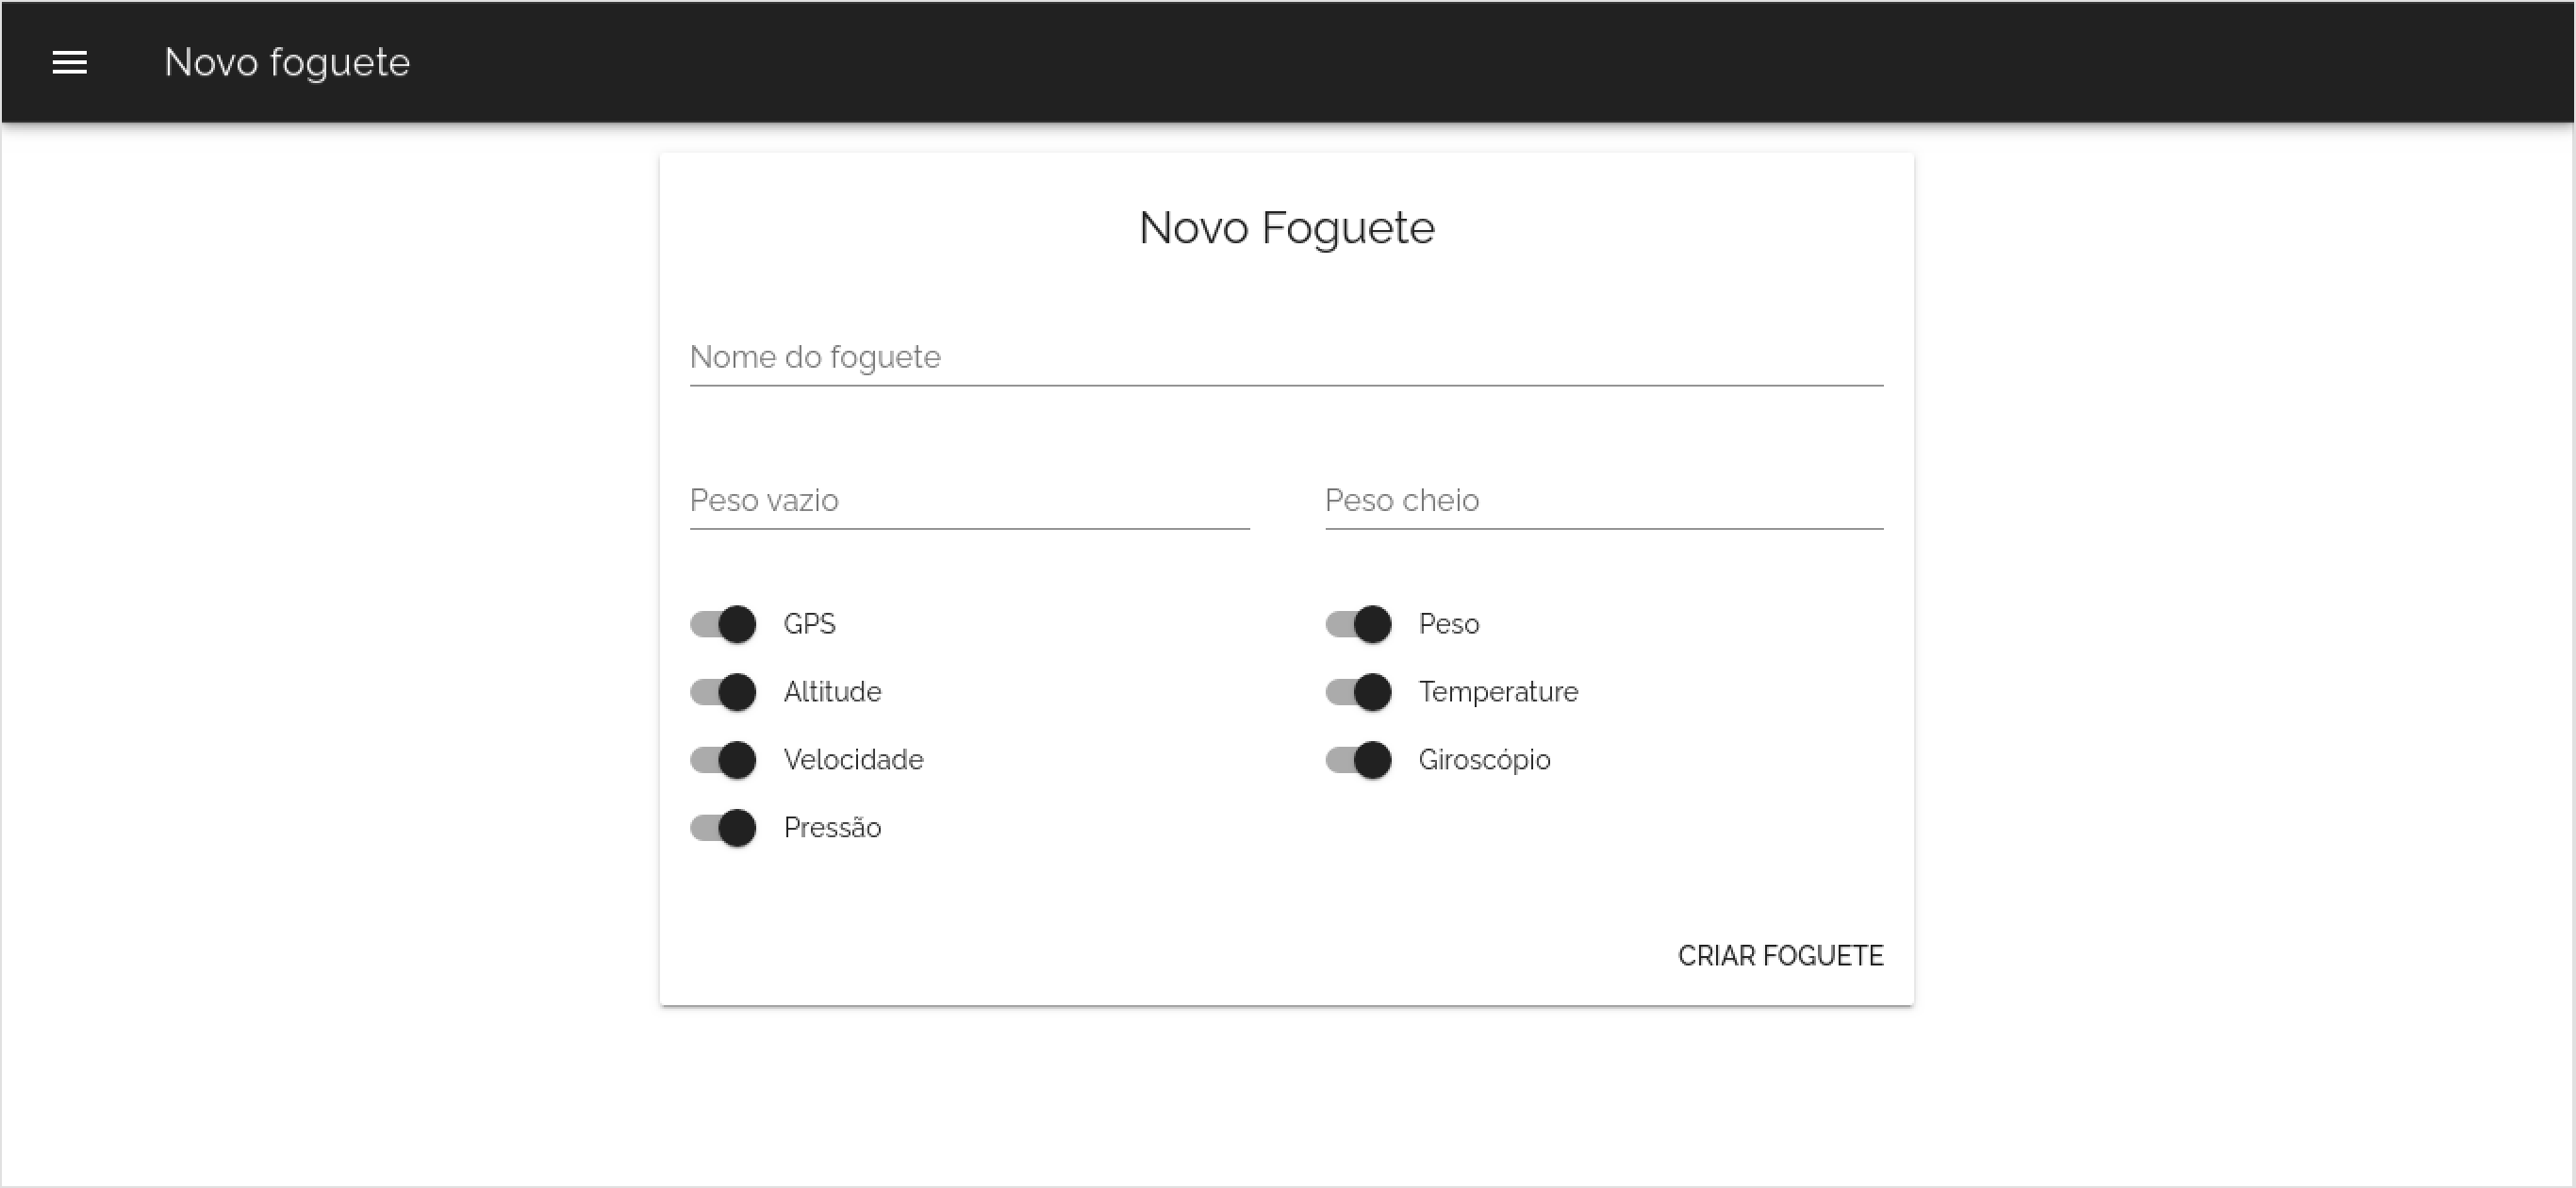
\includegraphics[width=\textwidth]{Figuras/telas/1.png}
        \label{teladecriacao}
	\caption{Tela de criação de novo foguete}
\end{figure} 
\end{center}

Na Figura \ref{teladehardware}, constata-se que após criar um novo foguete, o usuário pode adicionar os hardwares subsequentes que estão ligados ao foguete. Deve-se atentar para preencher corretamente os dados, caso não preencha os campos preenchidos incorretamente serão destacados na tela.
\begin{center}
    \begin{figure}[H]
\centering					    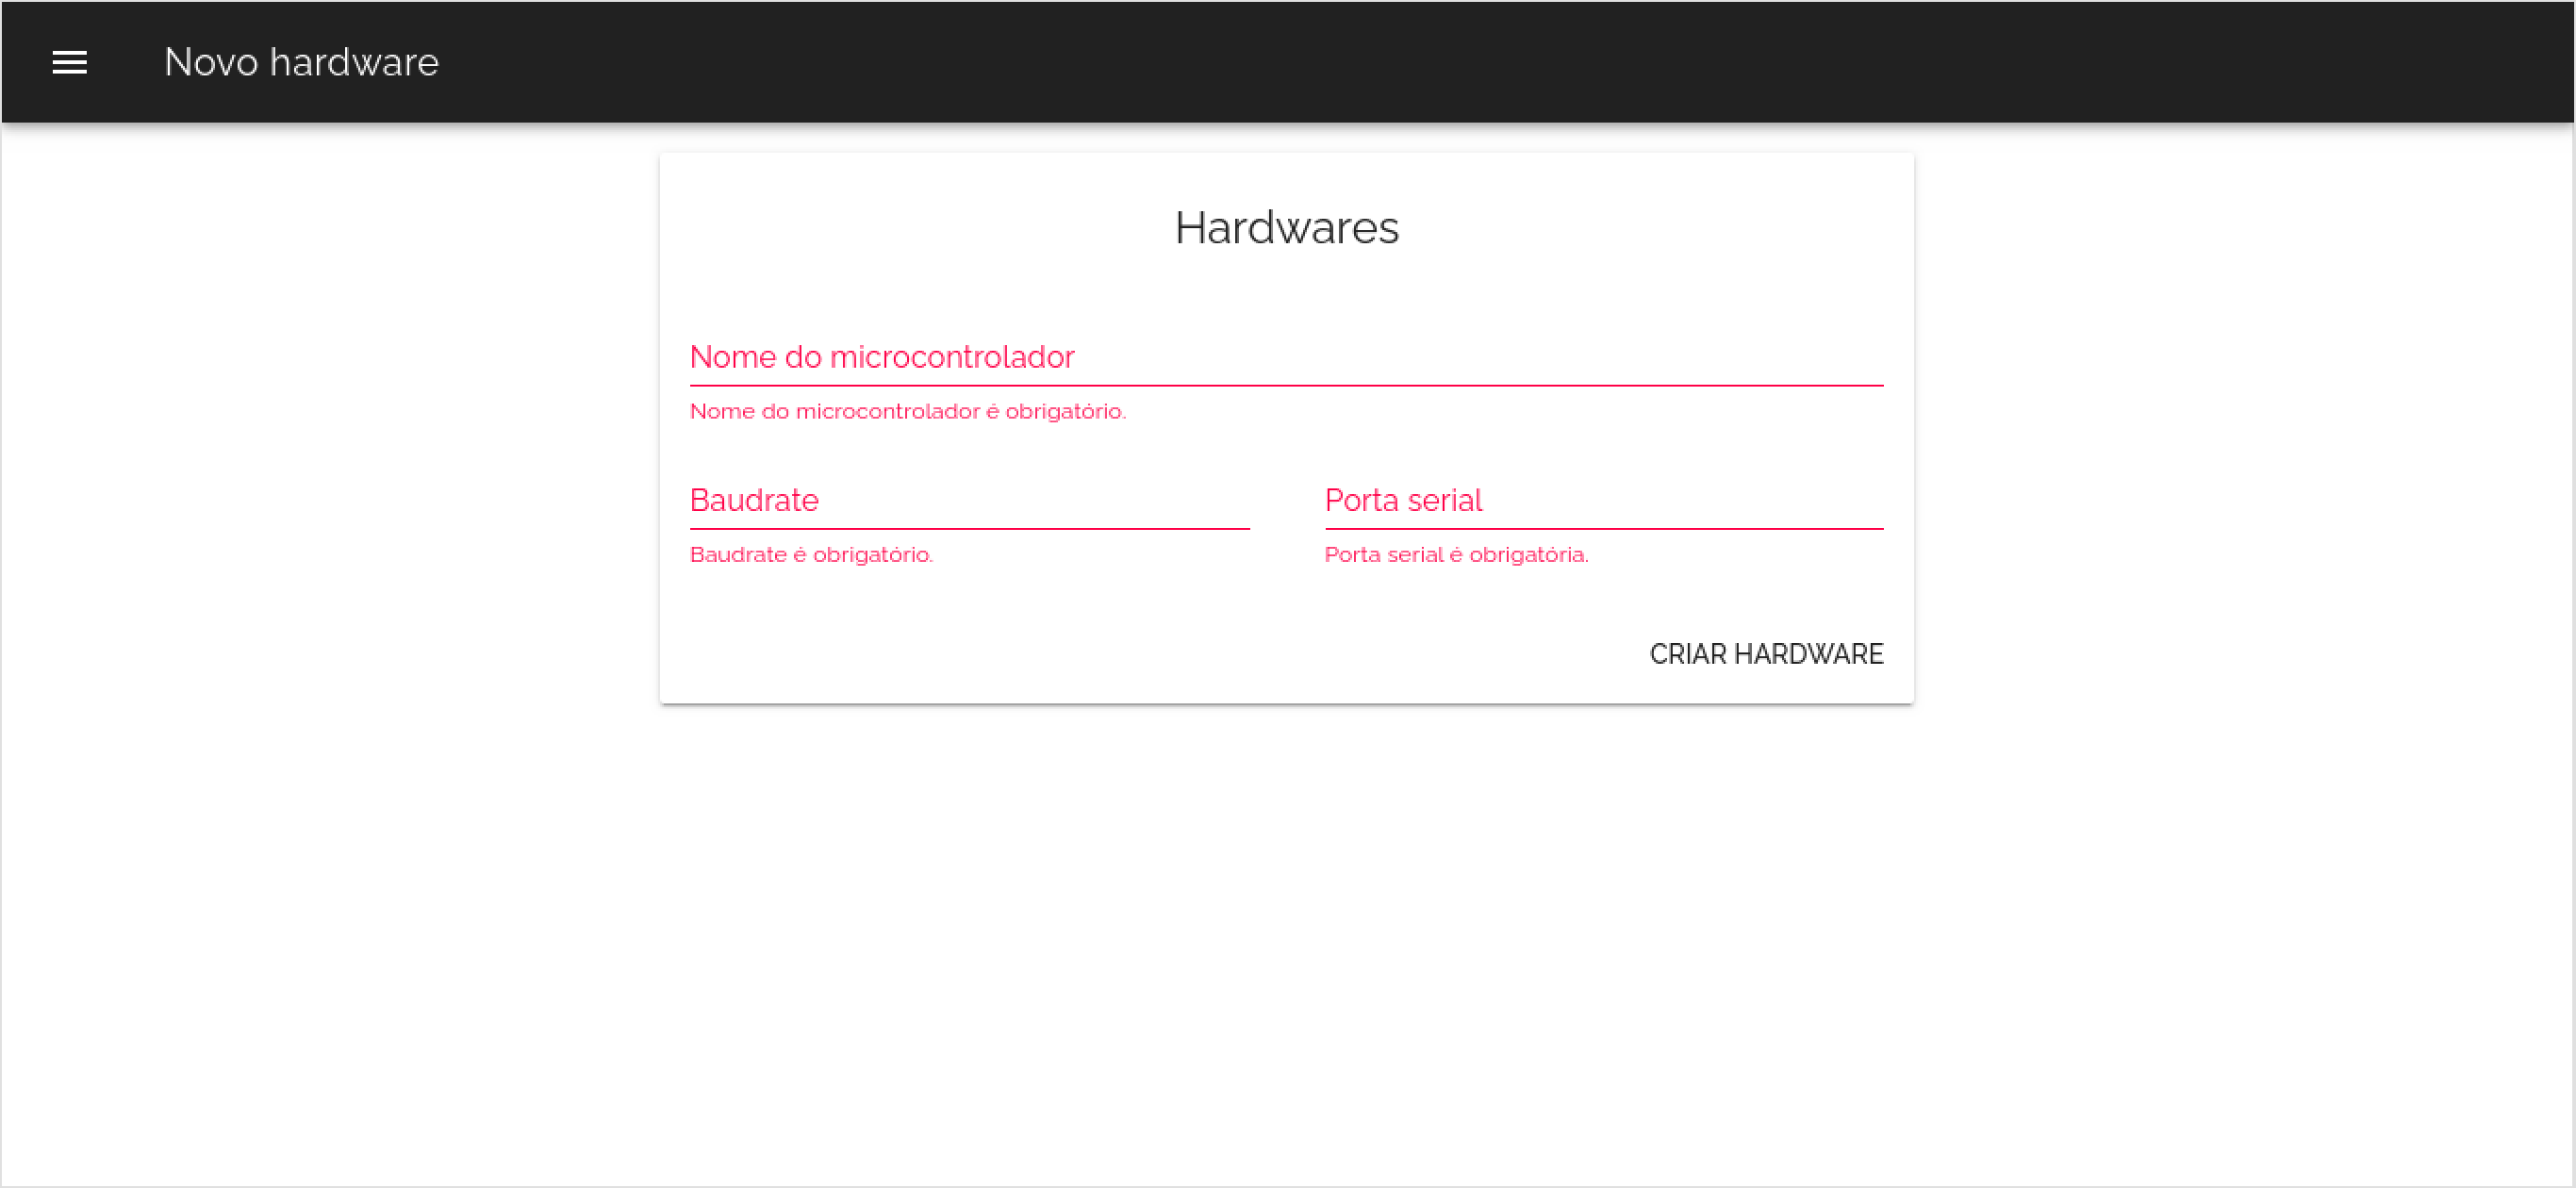
\includegraphics[width=\textwidth]{Figuras/telas/2-error.png}
        \label{teladehardware}
	\caption{ Tela de inserção de hardware}
\end{figure} 
\end{center}


A partir do menu, comandos também podem ser adicionados a partir da Figura \ref{teladecomando}. 
\begin{center}
\begin{figure}[H]					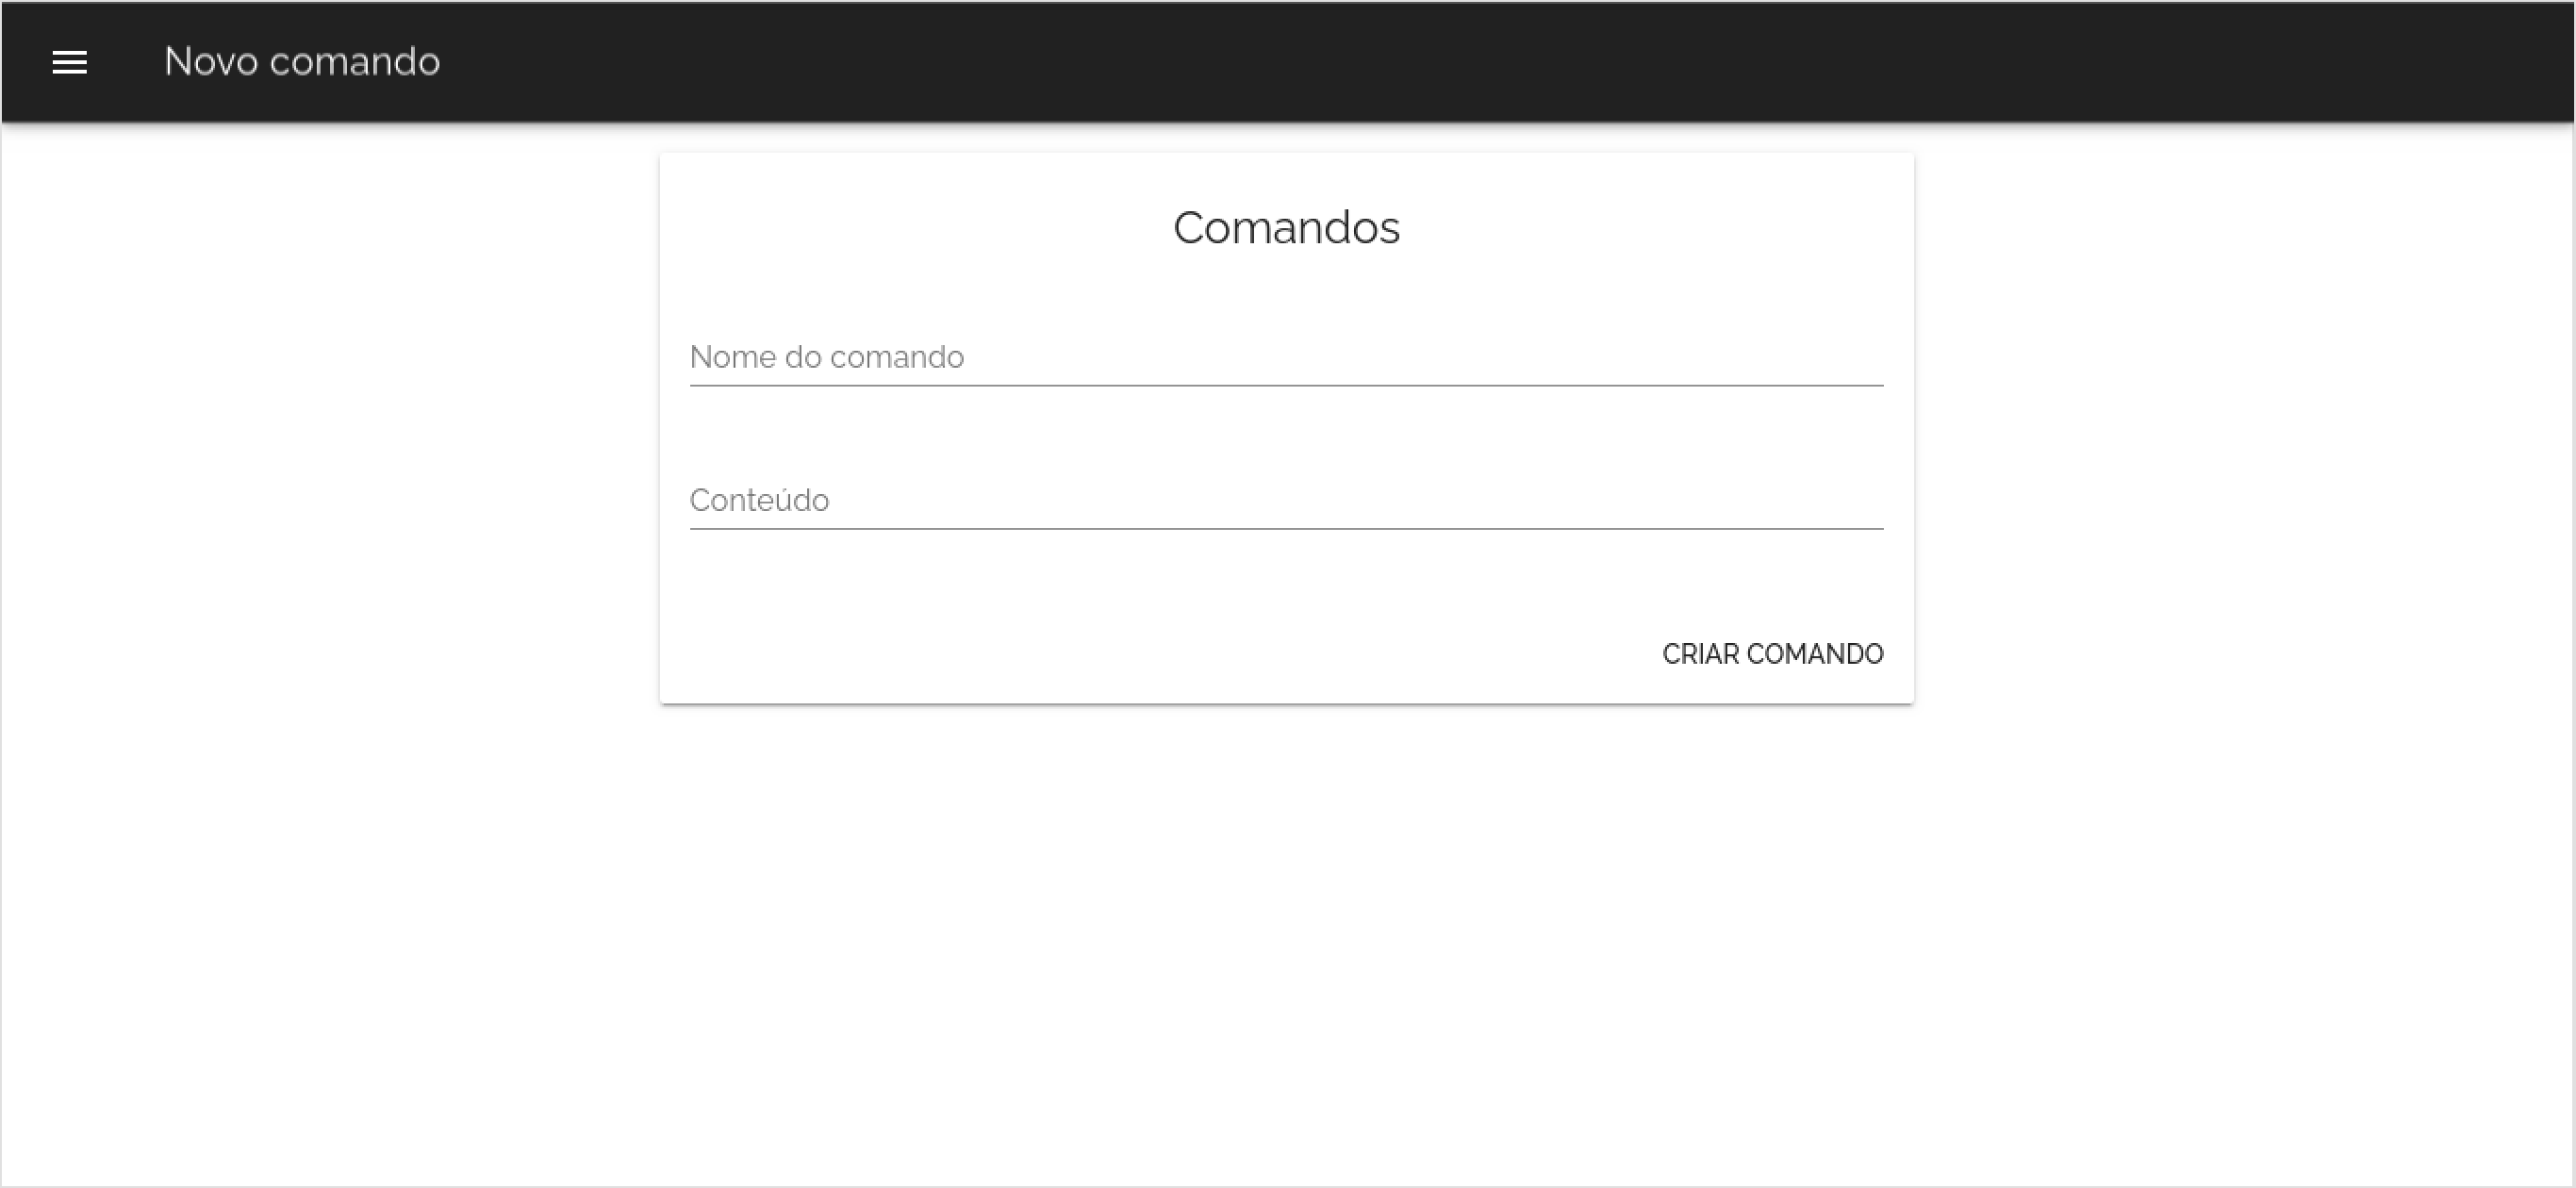
\includegraphics[width=\textwidth]{Figuras/telas/3.png}
        \label{teladecomando}
	\caption{Tela de novo comando}
\end{figure} 
\end{center}

Como pode-se observar na Figura \ref{telanovamissao}, para cadastrar uma nova missão selecione a opção Nova missão e preencha os dados conforme indicado. Após isso, clique em 'pŕóximo' para ir para a Figura \ref{telainiciarmissao} e selecionar qual foguete deseja designar para a missão.
\begin{center}
    

\begin{figure}[H]					
\includegraphics[width=\textwidth]{Figuras/telas/4.png}
        \label{telanovamissao}
	\caption{ Tela de nova missão}
\end{figure} 
\end{center}


\begin{center}
    

\begin{figure}[H]					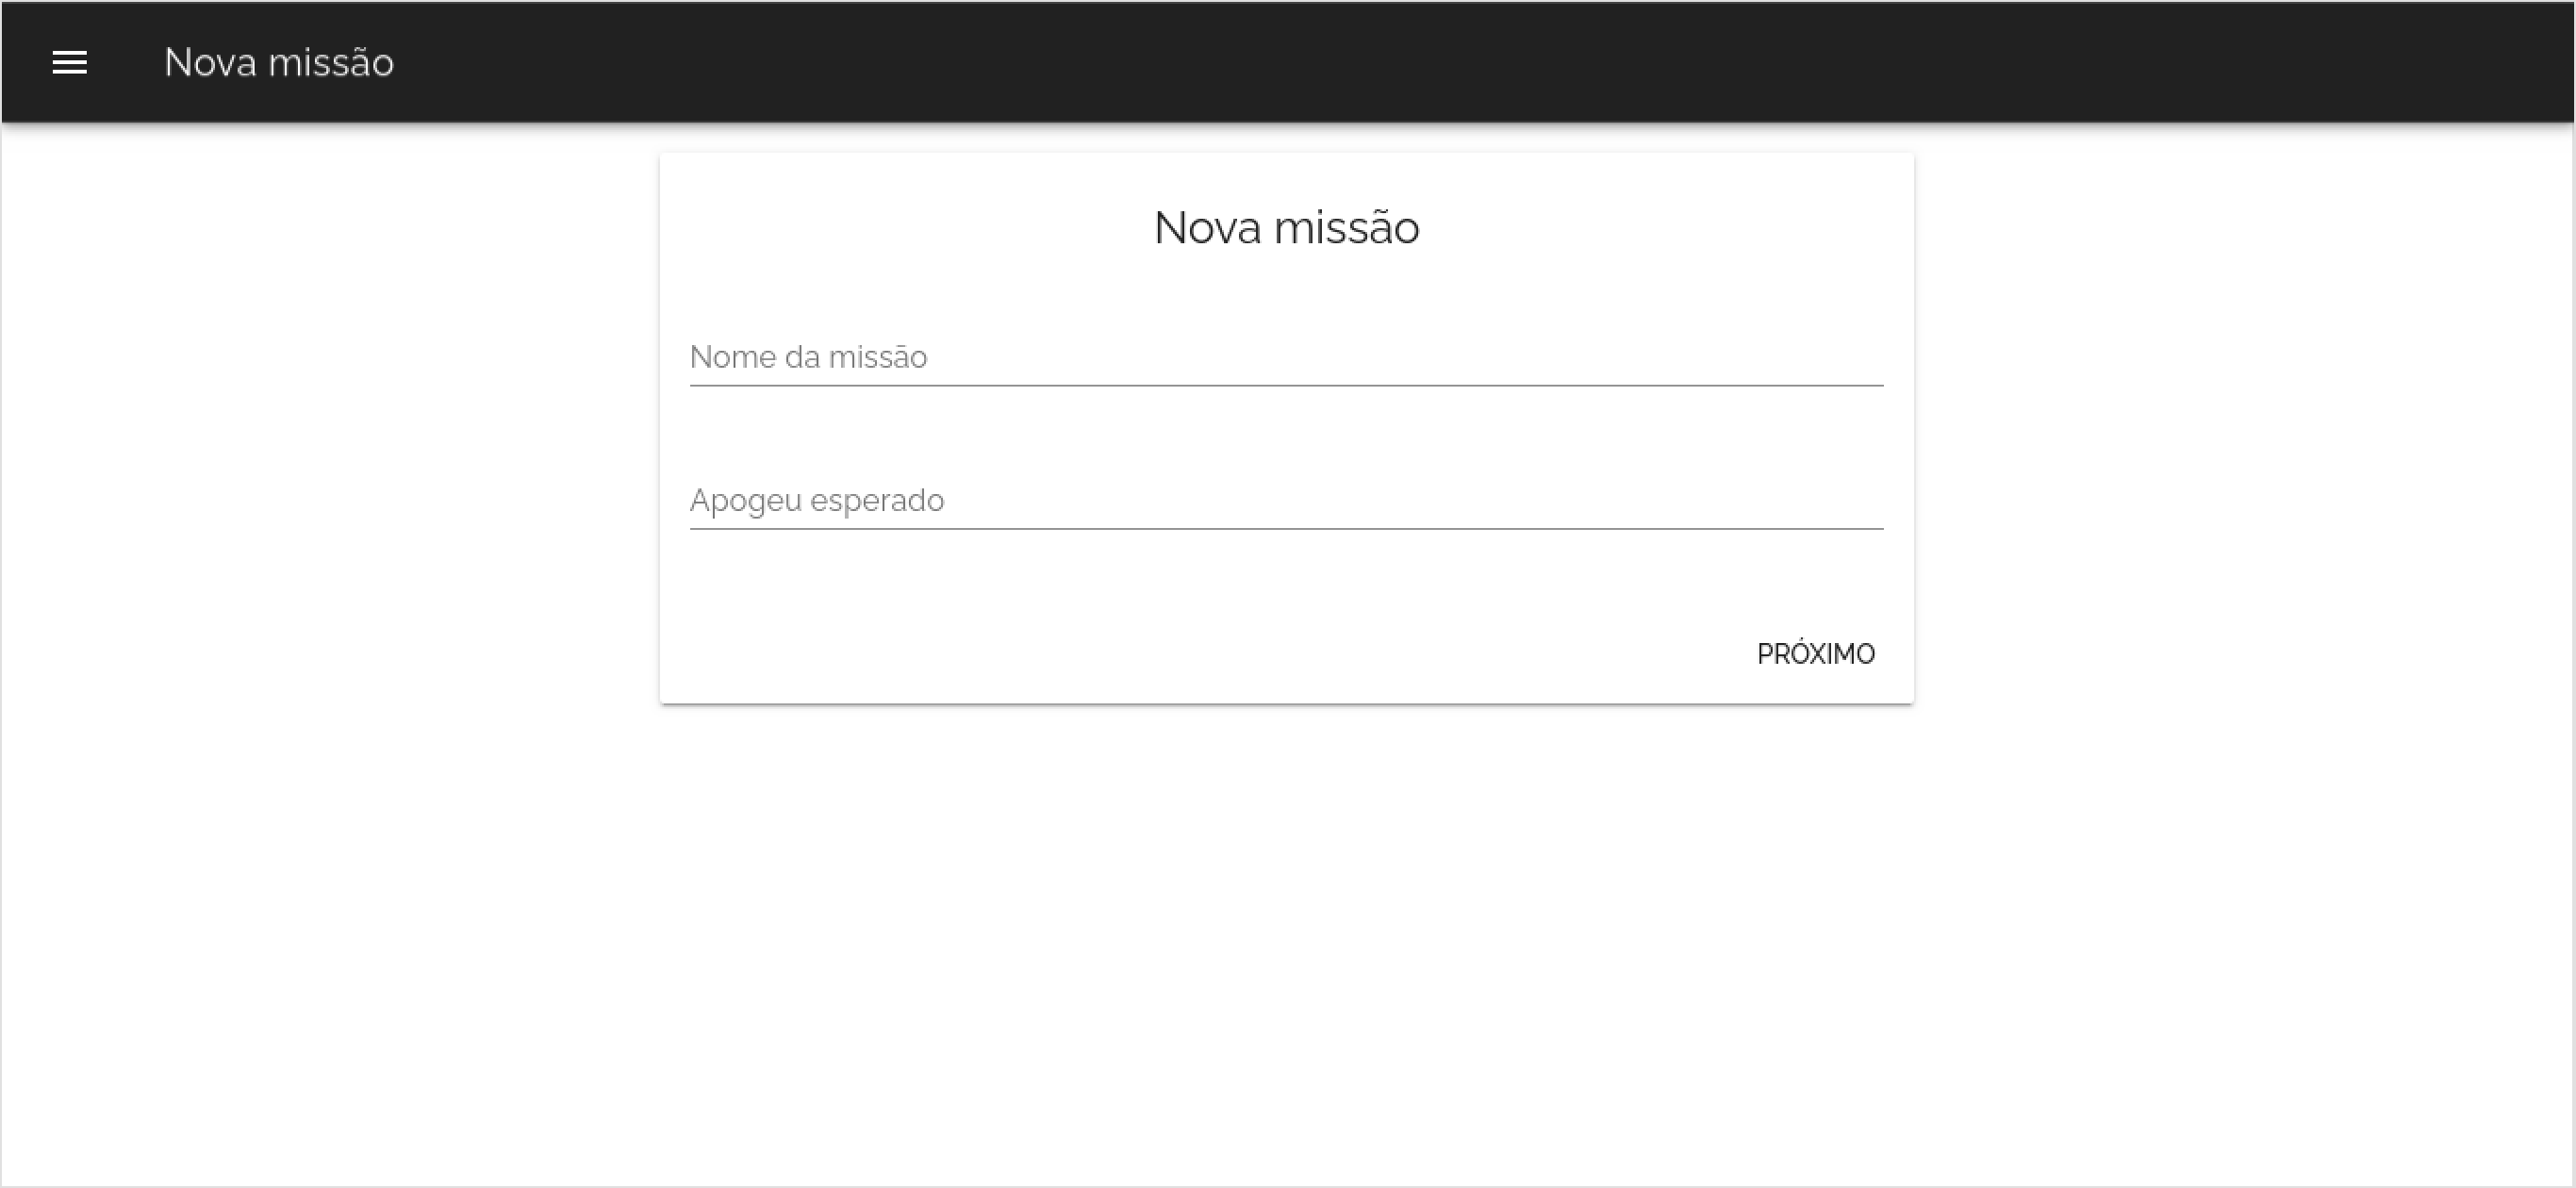
\includegraphics[width=\textwidth]{Figuras/telas/5.png}
        \label{telainiciarmissao}
	\caption{ Tela de iniciar missão}
\end{figure} 
\end{center}